\documentclass[10pt,a4paper]{article}
\usepackage[utf8]{inputenc}
\usepackage[spanish]{babel}
\usepackage{amsmath}
\usepackage{amsfonts}
\usepackage{amssymb}
\usepackage{graphicx}
\usepackage{listings}

\begin{document}
\begin{large}
\textbf{Tarea 4}
\end{large}

\section{Pregunta 01}

\begin{itemize}
\item[A] Factoriza 35 tratando de calcular 3Q.\vspace{.3cm}

Primero para poder realizar esta operación tenemos que enontrar 2Q, para ello tenemos que sumar los puntos (15,4) + (15,4) Recordando que la suma se define de la siguiente forma\vspace{.3cm}

P+Q=\[
\begin{cases}
Infinito  & \text{SI }  x_1=x_2 \ \&  -y_1= y_2 ;\\
(x_3,y_3) &  \text{} x_3= (\lambda^2 -x_1 - x_2)\  mod \ p \  y\  y_3 = (\lambda (x_1-x_3)-x_1)\ mod \ p\\

\end{cases}
\]  
Pero para esto necesitamos sacar primero a $\lambda$ que recordemos que se difine de la siguiente manera\vspace{.3cm}

 $\lambda$=\[
\begin{cases}
((3x_1^2+A) *  2(y_1)^{-1})) \ mod \ p & \text{si } P=Q ;\\
((y1-y2)*(x_1 - x_2))\ mod \ p & \text{si } P!=Q;\\

\end{cases}
\]

Para esto entonces simplemente sustituimos los valores, en lambda debido a que P=Q entonces usamos el primer caso de la lamda lo cual nos dice que $\lambda$ =
$(((3(15)^2)+-20) *  2(-4)^{-1}))mod 35$\\
$\rightarrow$ (((3*225)-20* (-8)$^{-1}$)mod 35\\
$\rightarrow$  ((675-20)*13)mod 35\\
 $\rightarrow$ (655 * 13) mod 35\\
  $\rightarrow$ 8515 mod 35\\
   $\therefore$ $\lambda = $  10\vspace{.3cm} 
   
 Ahora ya podemos sumar, primero sacaremos $x_3$ = $10^2$-15-15 mod 35 \\
 $\rightarrow$ 100-30 mod 35\\
 $\rightarrow$70 mod 35\\
 $\therefore$ x3=0\vspace{.3cm}
 
 Ahora debemos sacar a $y_3$=(10(15-0)- -4) mod 35 \\
 $\rightarrow$ 150+4 mod 35\\
 $\rightarrow$ 154 mod 35\\
$\therefore$ $y_3$ = 14  

Entonces ya sabemos el valor del punto 2Q, ahora debemos sumar Q+2q para tener 3Q, para eso debemos calcular de nuevo $\lambda$ por lo que haremos\vspace{.3cm}
$\lambda$= $\frac{-4-14} {15-0}$\vspace{.3cm}

Aquí encontramos un error debido a que 15 no tiene inverso multiplicativo en el grupo 35 así que eso implica que tenemos que sacar el MCD(35,15) = 5 $\therefore$ 5 es factor de 35.

\item[2] Factoriza 35 tratando de calcular 4Q duplicándolo.

Ahora no calcularemos 2Q debido a que ya lo calculamos anteriormente en el ejercicio 1 por lo cual pasaremos a calcular $\lambda$ bajo la definición del ejercicio 1\vspace{.3cm} 

$\lambda$= $\frac{3(0)^2}{2(14)}$mod 35 \vspace{.3cm}

Encontramos de nuevo el mismo problema que en el ejercicio anterior debido a que 28 mod 35  no tiene inverso, por lo cual debemos sacar su MCD(28,35) = 7 $\therefore$ 7 es un factor de 35 

\item[3] Calcula 3Q y 4Q sobre E (mod 5) y sobre E (mod 7) explica por que el factor 5
se obtiene calculando 3Q y por que el factor 7 se obtiene calculando 4Q.

Debido a que cuando calculas 3Q , intentamos sacar el inverso de 15 en el grupo 35, esto conflictuá ya que como 15 y 35 no son primos $\rightarrow$ que son números compuesto por primos esto nos lo sabemos por el teorema fundamental de la aritmética , ahora al sacar su MCD descubrimos que 5 es ese número $\therefore$ por esa razón 3 q , nos dio el valor 5 por compartir ese primo con 15 y análogamente pasa lo mismo con 28 y 35 

Ahora el valor de 3 Q con 5 =  No se puede calcular debido a que tenemos que cuando intentamos sumar Q= (15,-4) con 2Q=(0,4)(Los calculos de como se llego a 2q  se dejan como ejercicio para el lector ) e intentamos sacar $\alpha$ = (-4-4).(0-15)$^{-1}$\\
$\rightarrow$ 8 . (-15)$^{-1}$ y como -15 no esta en el campo de 5 entonces lo que hacemos es devolverlo con la operación modulo $\rightarrow$ -15 mod 5 = 0 y 0 no tiene inverso multiplicativo en 5  por lo que nuestro proceso termina aquí.\vspace{.3cm}

Ahora sacaremos el punto 4 Q sumando 2Q + 2Q lo sacamos la $\lambda$=3, haciendo los cálculos llegamos a que $x_3 =0 \land y_3= 4$ $\therefore$ Q3 = (0,4)\vspace{.3cm}

Nos falta sacar los valores de 3Q y 4Q en el modulo 7 por lo que tenemos que calcular 2Q al igual que tratamos al modulo 5 los calculos se dejaran al lector, entonces llegamos a 2Q=(0,0) por lo que ahora   pasamos a sumar Q=(15,-4) + 2Q=(0,0)  llegamos a que $\lambda$ = 3  por lo que $x_3$=1 y $y_3$ = 4, $\therefore$ $Q_3$ = (1,4) \vspace{.3cm}

Para finalizar solo nos falta calcular a 4Q por lo que tenemos que sumar 2Q + 2Q, pero esta no se puede debido a que cuando queremos calcular la $\lambda$ llegamos a los siguiente = (3(0)$^2$-20 * $(2*0)^{-1}$ ) y ya que no podemos sacar el inverso de 0 mod 7 debido a que no existe  \vspace{.3cm}    

\end{itemize}

\section{Pregunta 2}

Sea E la curva elíptica $y^2=x^3 + x +28 $ mod 71 definida sobre $Z_{71}$
 
\begin{itemize}
\item[a] Calcula y muestra el número de puntos de a
Para este ejercicio utilizamos un programa auxiliar de python debido a que este campo es de 71, eso implicaría calcular 71 puntos lo cual llevaría demasiado tiempo.\vspace{.3cm}

Por lo cual con ayuda de una clase de python que creamos para el proyecto 3 de python  creamos este método que nos ayudo a hacer esos cálculos
\begin{center}

\begin{figure}
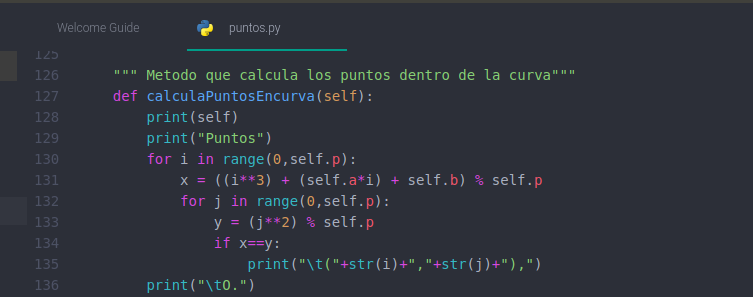
\includegraphics[width=0.7\textwidth]{Ejemplo1.png}
\caption{Método auxiliar que nos permite encontrar los puntos de una curva}
\label{fig:metoo auxiliar}
\end{figure} 
\end{center}	   
Entonces los puntos que nos devuelve son 
[ (1,32),   (1,39),   (2,31),   (2,40),   (3,22),   (3,49),   (4,5),   (4,66),   (5,4),   (5,67),   (6,26),   (6,45),   (12,8),   (12,63),   (13,26),   (13,45),   (15,9),   (15,62),   (19,27),   (19,44),   (20,5),   (20,66),   (21,3),   (21,68),   (22,30),   (22,41),   (23,19),   (23,52),   (25,22),   (25,49),   (27,0),   (31,32),   (31,39),   (33,1),   (33,70),   (34,23),   (34,48),   (35,14),   (35,57),   (36,12),   (36,59),   (37,33),   (37,38),   (39,32),   (39,39),   (41,7),   (41,64),   (43,22),   (43,49),   (47,5),   (47,66),   (48,11),   (48,60),   (49,24),   (49,47),   (52,26),   (52,45),   (53,0),   (58,27),   (58,44),   (61,15),   (61,56),   (62,0),   (63,17),   (63,54),   (65,27),   (65,44),   (66,18),   (66,53),   (69,35),   (69,36),'] Sin olvidar que además tenemos el punto $O$ por lo cual tenemos 72 distintos puntos :V 

\item[2] Muesttra que E no es un grupo cíclico.

\item[3] ¿Cuál es el máximo orden de un elemento en E? Encuentra un elemento que tenga dicho orden.

Por definición, el orden de un punto P en una Curva , es el entero más grande n $\in$ $Z_p$ donde p =71 (en este caso)   tal que nP = $O$, por lo que lo que debemos encontrar es
n max = max $\{  n|  nP = O , \forall P \in E \}$

Para esto tendremos que ir sumando los puntos que encontramos en la pregunta 2 a, hasta hallar un número tal que su orden sea 72 (el maximo orden posible) entonces con ayuda de este script  en python verificamos uno a uno los puntos a ver cual nos da ese orden 
 y vemos que un culpo que cumple eso es  (21,68)

\begin{center}

\begin{figure}
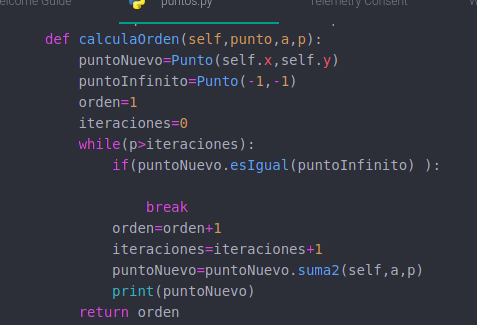
\includegraphics[width=0.7\textwidth]{Ejemplo2.png}
\caption{Método auxiliar que nos permite encontrar el orden de un punto}
\label{fig:metoo auxiliar}
\end{figure} 
\end{center}	

\end{itemize}

\end{document}
